  {\large \fontB Description:}
  
  {\bf solCx} is a 2-dimensional analytical solution to the Stokes' flow  equations.
  The boundary conditions are free-slip everywhere on a unit domain. 
  There is a viscosity jump in the x direction at $x=x_c$.
  The flow is driven by a temperature field represented by the density, $\rho$, as follows:
  \begin{equation}
    \rho = -\sigma \sin (n_z \pi z) \cos (n_x \pi x).
  \end{equation}

 {\large \fontB Parameters:}
  
 The variable parameters of this solution are:
 \begin{itemize}
   \item{density parameter: $ \sigma $.}
   \item{viscosities: $\eta_A$ and $\eta_B$.}
   \item{viscosity jump location: $x_c$.}
   \item{wave number in z domain: $ n_z $. ($n_z$ may be non-integral)}
   \item{wave number in x domain: $ n_x $. ($n_x$ must be integral)}
 \end{itemize}

  \begin{SCfigure}[][h]
    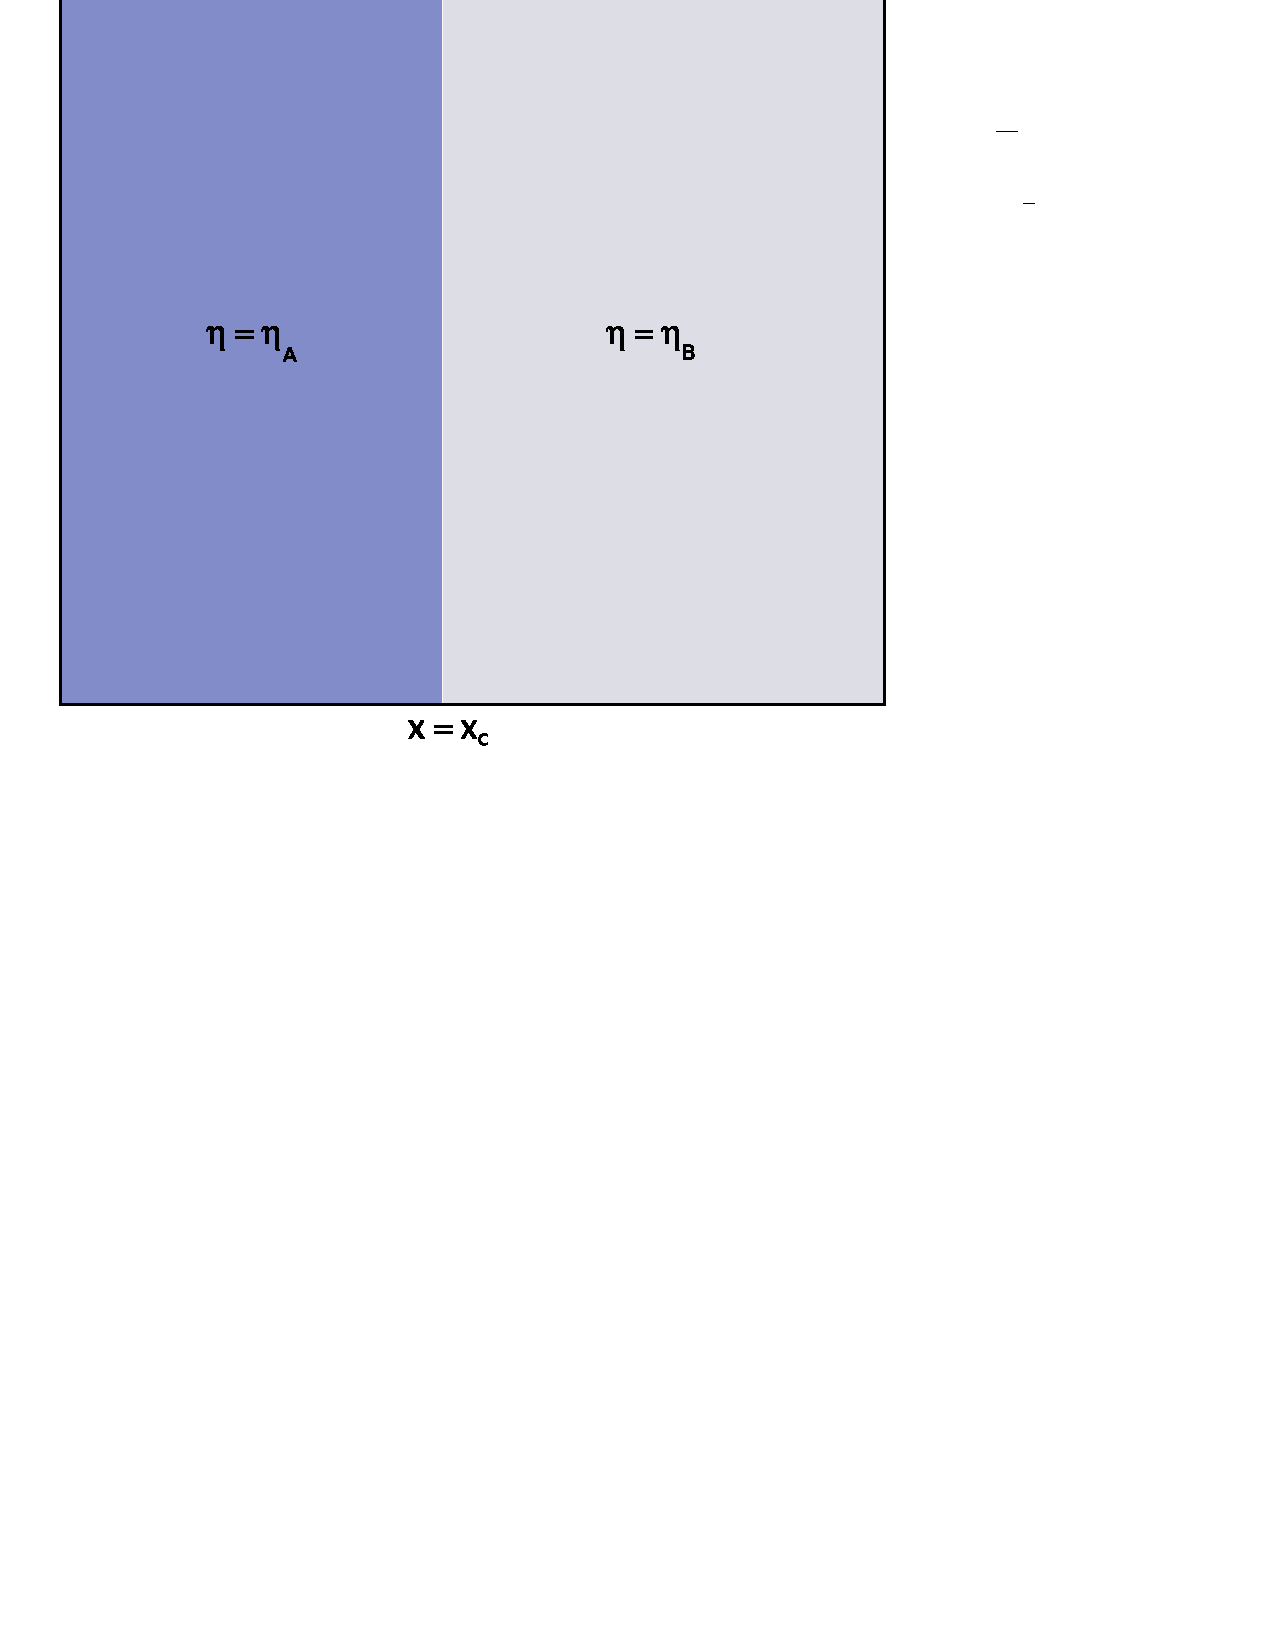
\includegraphics[width=6cm,clip]{../figs/figCx}
    \caption[Short caption]{\label{figCx} 
      Solution ({\bf solCx}):
      This solution has a box of density $\rho = -\sigma \sin (n_z \pi z) \cos (n_x \pi x)$ .
      It is has a viscosity jump at $x = x_c$.
      The boundary conditions are free slip everywhere on the surfaces of the unit box.}
  \end{SCfigure} 
  \vspace{-47mm}
  {\small
  \[
    \hspace{-77mm} \rho = -\sigma \sin (n_z \pi z) \cos (n_x \pi x)
  \]
  }  
  \vspace{47mm}
